\documentclass[11pt,a4paper]{moderncv}
\usepackage{pdfpages}
\usepackage{import} \import{./}{setup.tex}

\name{Federico}{del Mazo}
\title{
    \spa{Curriculum Vitae}
    \en{Résumé}
}
\address{Beruti 545, Ramos Mejía (1704)}
\phone[mobile]{+54 911 6110 1997}
\phone[fixed]{011 4656 4494}
\email{fdelmazo@fi.uba.ar}
\extrainfo{\href{https://www.linkedin.com/in/fdelmazo/}{\faLinkedin \vspace{0.4mm} FdelMazo} • \href{https://www.github.com/fdelmazo/}{\faGithub \vspace{0.4mm} FdelMazo}}
\quote{
    \spa{21 años, estudiante de Ingeniería en Informática.}
    \en{21 years old, Computer Engineering student.}
}

\begin{document}


\spa{
    \begin{textblock*}{1.51cm}(19cm,0.2cm) 
        \begin{shaded*}
        \centering
            \href{https://fdelmazo.github.io/CV/cv-en.pdf}{SPA}
        \end{shaded*}
    \end{textblock*}
}

\en{
    \begin{textblock*}{1.51cm}(19cm,0.2cm) 
        \begin{shaded*}
        \centering
            \href{https://fdelmazo.github.io/CV/cv-es.pdf}{ENG}
        \end{shaded*}
    \end{textblock*}
}

\begin{picture}(0,0)
\put(-30,-110){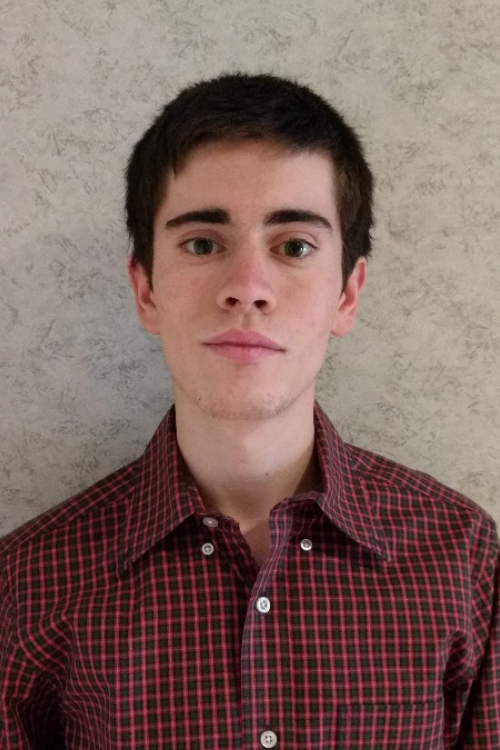
\includegraphics[scale=0.20]{fotoCV}}
\end{picture}

\thispagestyle{onlyfooter}

\makecvtitle
\addtolength{\parskip}{6pt}

\spa{Estudiante en busqueda de seguir desarrollandose en la industria y enriquecer sus conocimientos.}    
\en{Student eager to delve deep into the IT industry and looking forward to improve his knowledge and skills.}

\section{\spa{Experiencia Laboral}\en{Work Experience}}

\cventry
    {\spa{Abril 2018--Actualidad}\en{April 2018--Now}}
    {\spa{Desarrollador de software}\en{Full Stack developer}}
    {Raico S.A.}{}{}{\url{https://www.raiconet.com/}}

\section{\spa{Experiencia Laboral No Rentada}\en{Non-paid Work Experience}}

\cventry
    {\spa{Agosto 2017--Actualidad}\en{August 2017--Now}}
    {\spa{Ayudante de}\en{Adjunct professor in} Algoritmos y Programación II - Curso Wachenhauzer}
    {Universidad de Buenos Aires, Facultad de Ingeniería}{}{}{\url{https://algoritmos-rw.github.io/algo2/}}

\section{\spa{Educación}\en{Education}}

\cventry
    {\spa{2015--Actualidad}\en{2015--Now}}
    {\spa{Estudiante de Ingeniería en Informática}\en{Computer Engineering student}}
    {Universidad de Buenos Aires, Facultad de Ingeniería}{}{}{}

\cventry
    {2009--2014}
    {\spa{Bachiller Bilingüe en Economía y Administración}\en{Bilingual bachelors' degree in economics and business administration}}
    {Colegio Ward}{}{}{\textit{\spa{Promedio general}\en{Grade Point Average} 8.29}}

\cventry
    {2012--2013}
    {International General Certificate of Secondary Education (IGCSE)}
    {University of Cambridge}{}{}{\textit{Passed with Merit}}
%     Environtmental Management B
%     Geography B
%     First Language Spanish D
%     Economics B
%     Mathematics B
%     Business Studies C
%     First language english D

\cventry
    {2011}
    {First Certificate in English}
    {University of Cambridge}{}{}{\textit{Grade C}}
% Cambridge ESOL Level 1 Certificate in ESOL International

\section{\spa{Conocimientos específicos}\en{Specific skills}}

\begin{itemize}
\item \textbf{\spa{Lenguajes de programación}\en{Programming languages}:} C, Python, Java, JavaScript, Lua.
\item \textbf{\spa{Otros lenguajes}\en{Other languages}:} SQL, TeX, HTML, CSS.
\item \textbf{\spa{Otros}\en{Other}:} jQuery, Bootstrap, Groovy, Grails.
\end{itemize}

\IfFileExists{./notas.pdf}{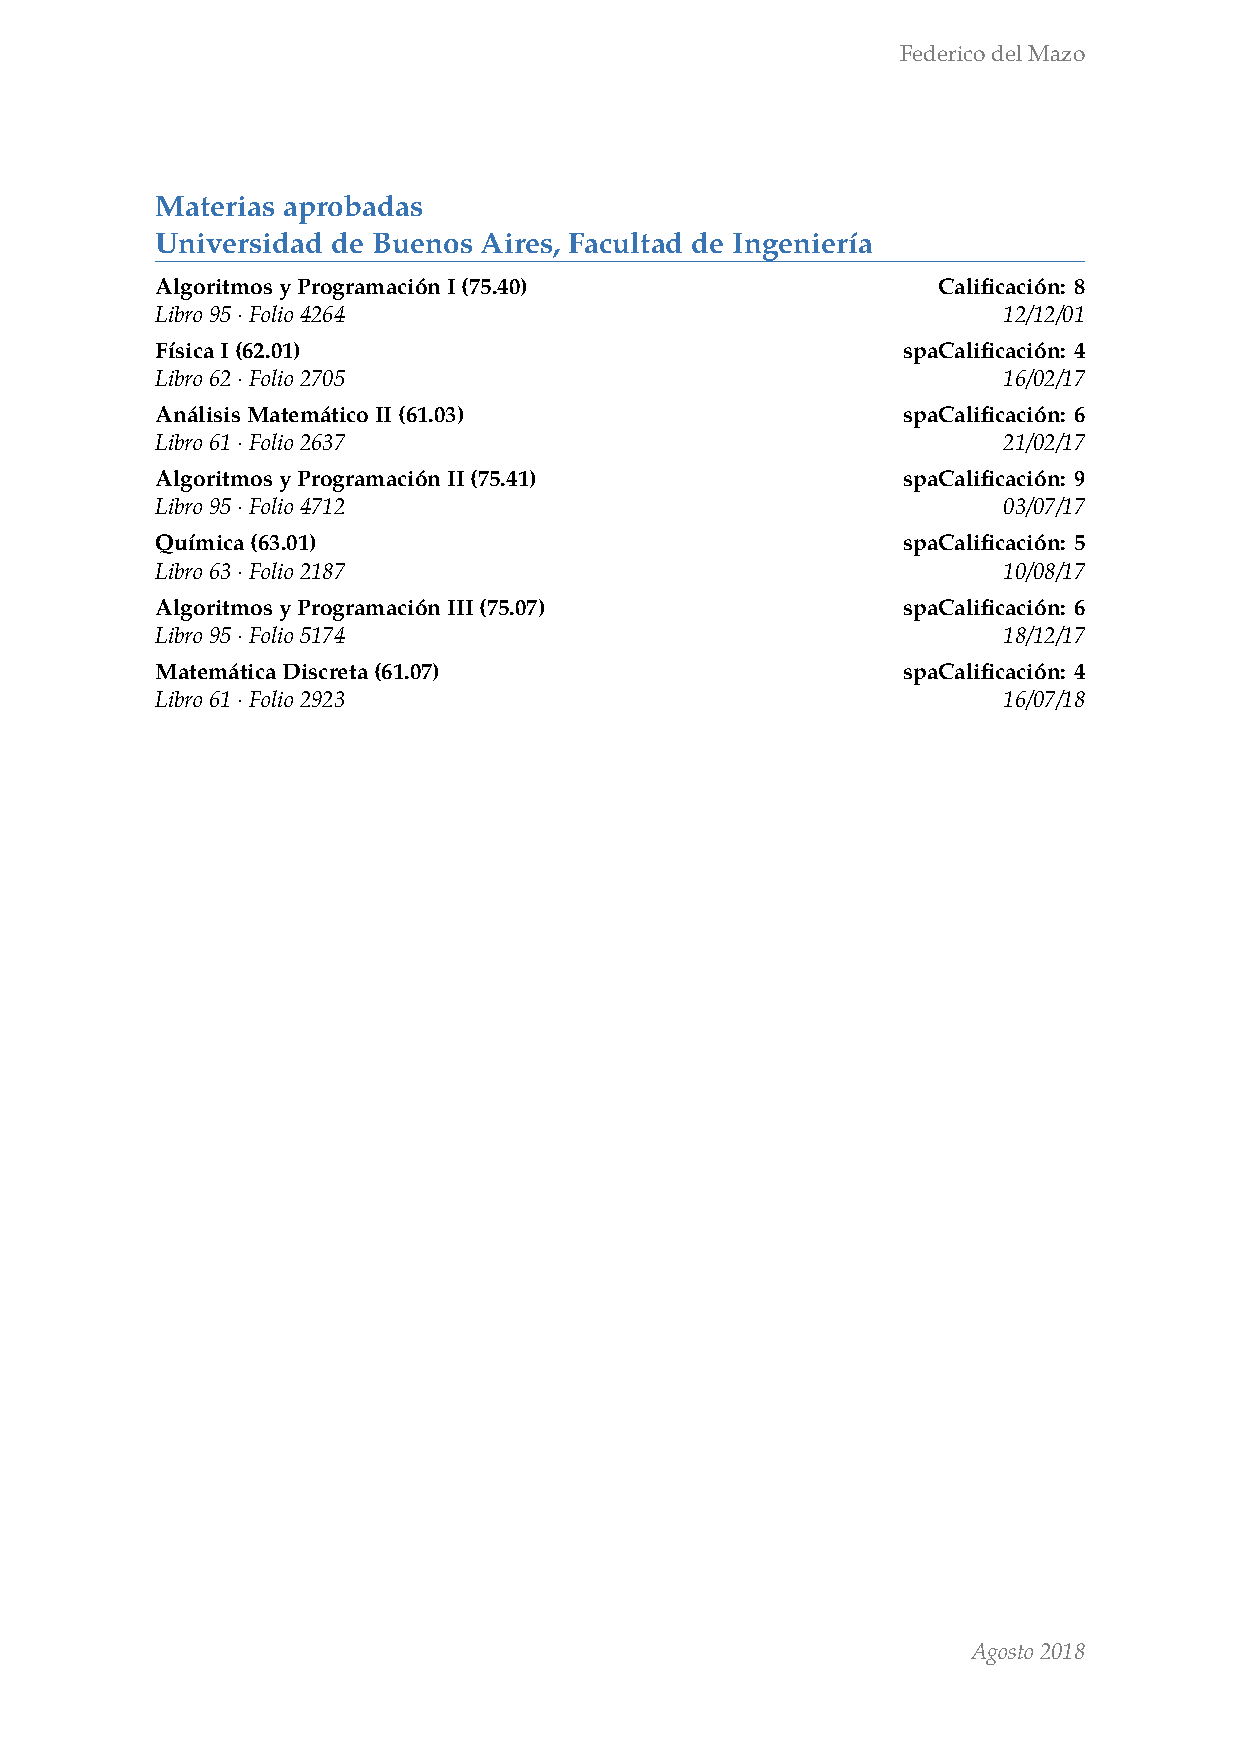
\includepdf[pages=-]{notas.pdf}}{}
\end{document}

